\documentclass[10pt]{article}

\usepackage{amsfonts, amsthm, amsmath, fullpage, tikz, wrapfig, enumerate}

\newcommand{\card}[1]{\left| #1 \right|}
\newcommand{\nat}{\mathbb{N}}
\newcommand{\ints}{\mathbb{•}
\newcommand{\reals}{\mathbb{R}}
\newcommand{\chtitle}[1]{\noindent \vspace{5mm}\textbf{Chapter #1}\vspace{3mm}}

\begin{document}
\begin{flushleft}
\textbf{\noindent
CS 341 Automata Theory \\
Geoffrey Parker - grp352 \\
Homework 8 \\
Due Tuesday, March 6}\\
\end{flushleft}
\noindent
This assignment covers Chapter 12. \\

\begin{enumerate}[1)]

% ---
% 1
% ---

\item
Build a PDA to accept each of the following languages $L$:
\begin{enumerate}[a)]
%a)
\item
$\{\texttt{a}^n\texttt{b}^m:\ m \leq n \leq 2m\}$.
\begin{proof}[Solution:]
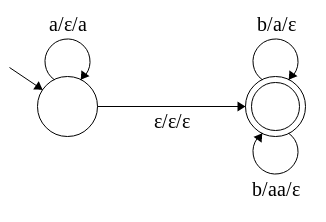
\includegraphics[scale=.5]{images/solutions/1a.png}
\end{proof}

%b)
\item
$\{w \in \{\texttt{a}, \texttt{b}\}^*$ : every prefix of $w$ has at least as many \texttt{a}'s as \texttt{b}'s\}.
\begin{proof}[Solution:] $ $\\
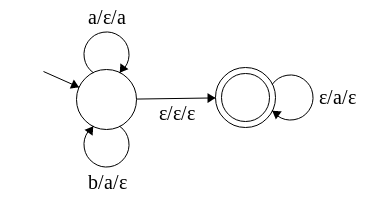
\includegraphics[scale=.5]{images/solutions/1b.png}
\end{proof}

%c)
\item
$\{\texttt{a}^n\texttt{b}^m:\ m \geq n, m-n$ is even\}.
\begin{proof}[Solution:] $ $\\
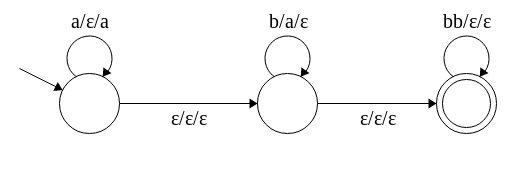
\includegraphics[scale=.5]{images/solutions/1c.png}
\end{proof}
\end{enumerate}

\pagebreak
%---
% 2
%---

\item
Let $L = \{\texttt{ba}^{m_1}\texttt{ba}^{m_2}\texttt{ba}^{m_3} \ldots \texttt{ba}^{m_n}:$ $n \geq 2$, $m_1, m_2, \ldots, m_n \geq 0$, and $m_i \neq m_j$ for some $i$, $j$\}.
\begin{enumerate}[a)]
%a
\item
Show a PDA that accepts $L$.
\begin{proof}[Solution:] $ $\\
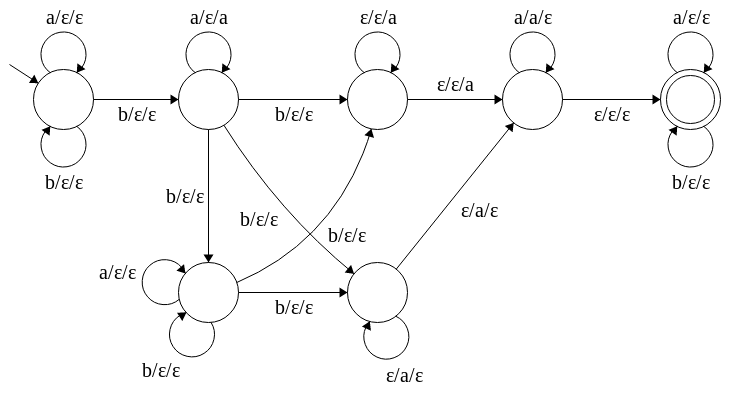
\includegraphics[scale=.5]{images/solutions/2a.png}
\end{proof}

%b
\item
Show a context-free grammar that generates $L$.
\begin{proof}[Solution:]
\begin{align*}
S &\rightarrow GS \mid SG \mid Y\\
Y &\rightarrow bL \mid bR\\
L &\rightarrow aLa \mid aL \mid aXb\\
R &\rightarrow aRa \mid Ra \mid Xba\\
X &\rightarrow GX \mid \epsilon\\
G &\rightarrow Ga \mid b
\end{align*}
\end{proof}

%c
\item
Prove that $L$ is not regular.
\begin{proof}[Proof:]
If $L$ were regular, then $L^R$ would be regular.  If $L^R$ were regular, then $(L^R)^c$ would be regular.  If $(L^R)^c$ were regular, then $L' = (L^R)^c$ \cap $a^*ba^*b$ would be regular. $L' = a^nba^nb$.
Let $w = a^{2k}ba^{4k}b$.
\end{proof}
\end{enumerate}

% ---
% 3
% ---

\item
Consider the language $L = L_1 \cap L_2$, where $L_1 = \{ww^R:\ w \in \{\texttt{a}, \texttt{b}\}^*\}$ and $L_2 = \{\texttt{a}^n\texttt{b}^*\texttt{a}^n:\ n \geq 0\}$.
\begin{enumerate}[a)]
%a
\item
List the first four strings in the lexicographic enumeration of $L$.
\begin{proof}[Solution:]
\texttt{$\epsilon$, aa, aaaa, abba}
\end{proof}

%b
\item
Write a context-free grammar to generate $L$.
\begin{proof}[Solution:]
\begin{align*}
S &\rightarrow aSa \mid B\\
B &\rightarrow bBb \mid \epsilon
\end{align*}
\end{proof}

%c
\item
Show a natural PDA for $L$.  (In other words, don’t just build it from the grammar using one of the two-state constructions presented in the book.)
\begin{proof}[Solution:]$ $\\
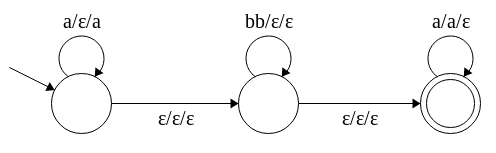
\includegraphics[scale=.5]{images/solutions/3c.png}
\end{proof}

%d
\item
Prove that $L$ is not regular.
\begin{proof}[Proof:]
Let $w = a^kbba^k$.  Then $y$ must be $a^p$ for some $p$ in the first group of $a$'s.  Now pump out and the new string is not in the language because the $a$'s are no longer balanced.
\end{proof}
\end{enumerate}


% ---
% 4
% ---

\item
* Let $L = \{w \in \{\texttt{a}, \texttt{b}\}^*$ : the first, middle, and last characters of $w$ are identical\}.
\begin{enumerate}[a)]
%a
\item
Show a context-free grammar for $L$.
\begin{proof}[Solution:]
\end{proof}

%b
\item
Show a natural PDA that accepts $L$.
\begin{proof}[Solution:]
\end{proof}

%c
\item
Prove that $L$ is not regular.
\begin{proof}[Proof:]
\end{proof}
\end{enumerate}
\end{enumerate}
\end{document}
